\documentclass{article}
\usepackage[left=2cm,right=2cm,top=2cm,bottom=2cm]{geometry}
\usepackage[utf8]{inputenc}
\usepackage[german]{babel}
\usepackage{amsmath}
\usepackage{dsfont}
\usepackage[export]{adjustbox}
\usepackage{amsthm}
\usepackage{color}
\usepackage{amsfonts}
\usepackage{amssymb}
\usepackage{wasysym}
\usepackage{makeidx}
\usepackage{graphicx}
\usepackage[colorlinks=true,urlcolor=blue,linkcolor=blue]{hyperref}
\usepackage{ziffer}
\usepackage{minted}
\usepackage{xcolor}
\usepackage{framed}
\usepackage{mdframed}
\usepackage{subfiles}
\usemintedstyle{emacs}

\definecolor{purp}{HTML}{9A72AC}
\definecolor{re}{HTML}{FC6255}
\definecolor{gre}{HTML}{83C167}
\definecolor{blu}{HTML}{58C4DD}
\definecolor{shadecolor}{rgb}{0.85,0.85,0.85}
\definecolor{bg}{rgb}{0.95,0.95,0.95}
\setlength{\parindent}{0em} 

\BeforeBeginEnvironment{minted}{\begin{mdframed}[linewidth =2 ,backgroundcolor=bg , linecolor=black, linewidth=0.5]}
\AfterEndEnvironment{minted}{\end{mdframed}}

\newtheorem{defi}{Definition}
\BeforeBeginEnvironment{defi}{\begin{mdframed}[linewidth =2 ,backgroundcolor=bg , linecolor=black, linewidth=0.5]}
\AfterEndEnvironment{defi}{\end{mdframed}}

\newcommand{\bsp}{\textbf{Beispiel}:}
%\newcommand{\task}{\textbf{Aufgabe}:}

\newcommand{\bol}[1]{\textbf{#1}}
\newcommand{\q}[1]{\glqq #1\grqq}
\newcommand{\DODO}[1]{\textbf{\textcolor{red}{DODO:}} #1 \\ \begin{center}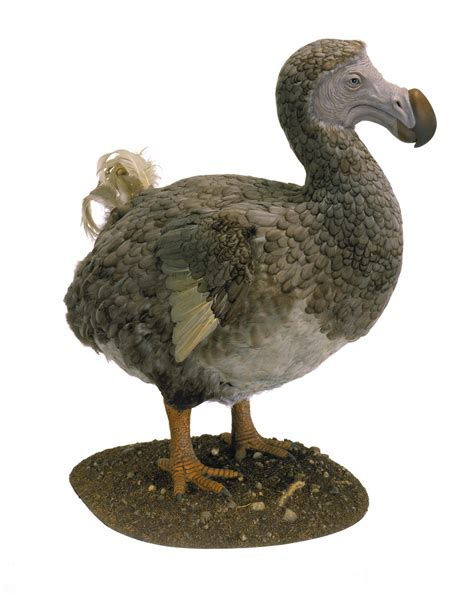
\includegraphics[scale=0.2]{../../media/dodo.jpg} \end{center}}

\newenvironment{task}[1]{
    \begin{shaded*}
    \textbf{Aufgabe #1}:
}{
    \end{shaded*}
}

\begin{document}
Lösungen zu den Aufgaben)\\
\textbf{Aufgabe 2}:
Mit unseren Vorarbeiten (insbesondere das Entfernen der Nachfolger-Referenz der Wurzel) ist diese Aufgabe sehr leicht. 
Die Wurzel die entfernt wird, wird mit der normalen hintenAnfügen() Methode wieder eignefügt. 
\begin{minted}{Java}
    //class Human 
    public void setNext(Human human) {
        next human;
    }
    //class MyListLinked
    public void moveToBack(){
        this.push(this.pop());
    }
\end{minted}
Graphisch veranschaulicht:
\begin{center}
    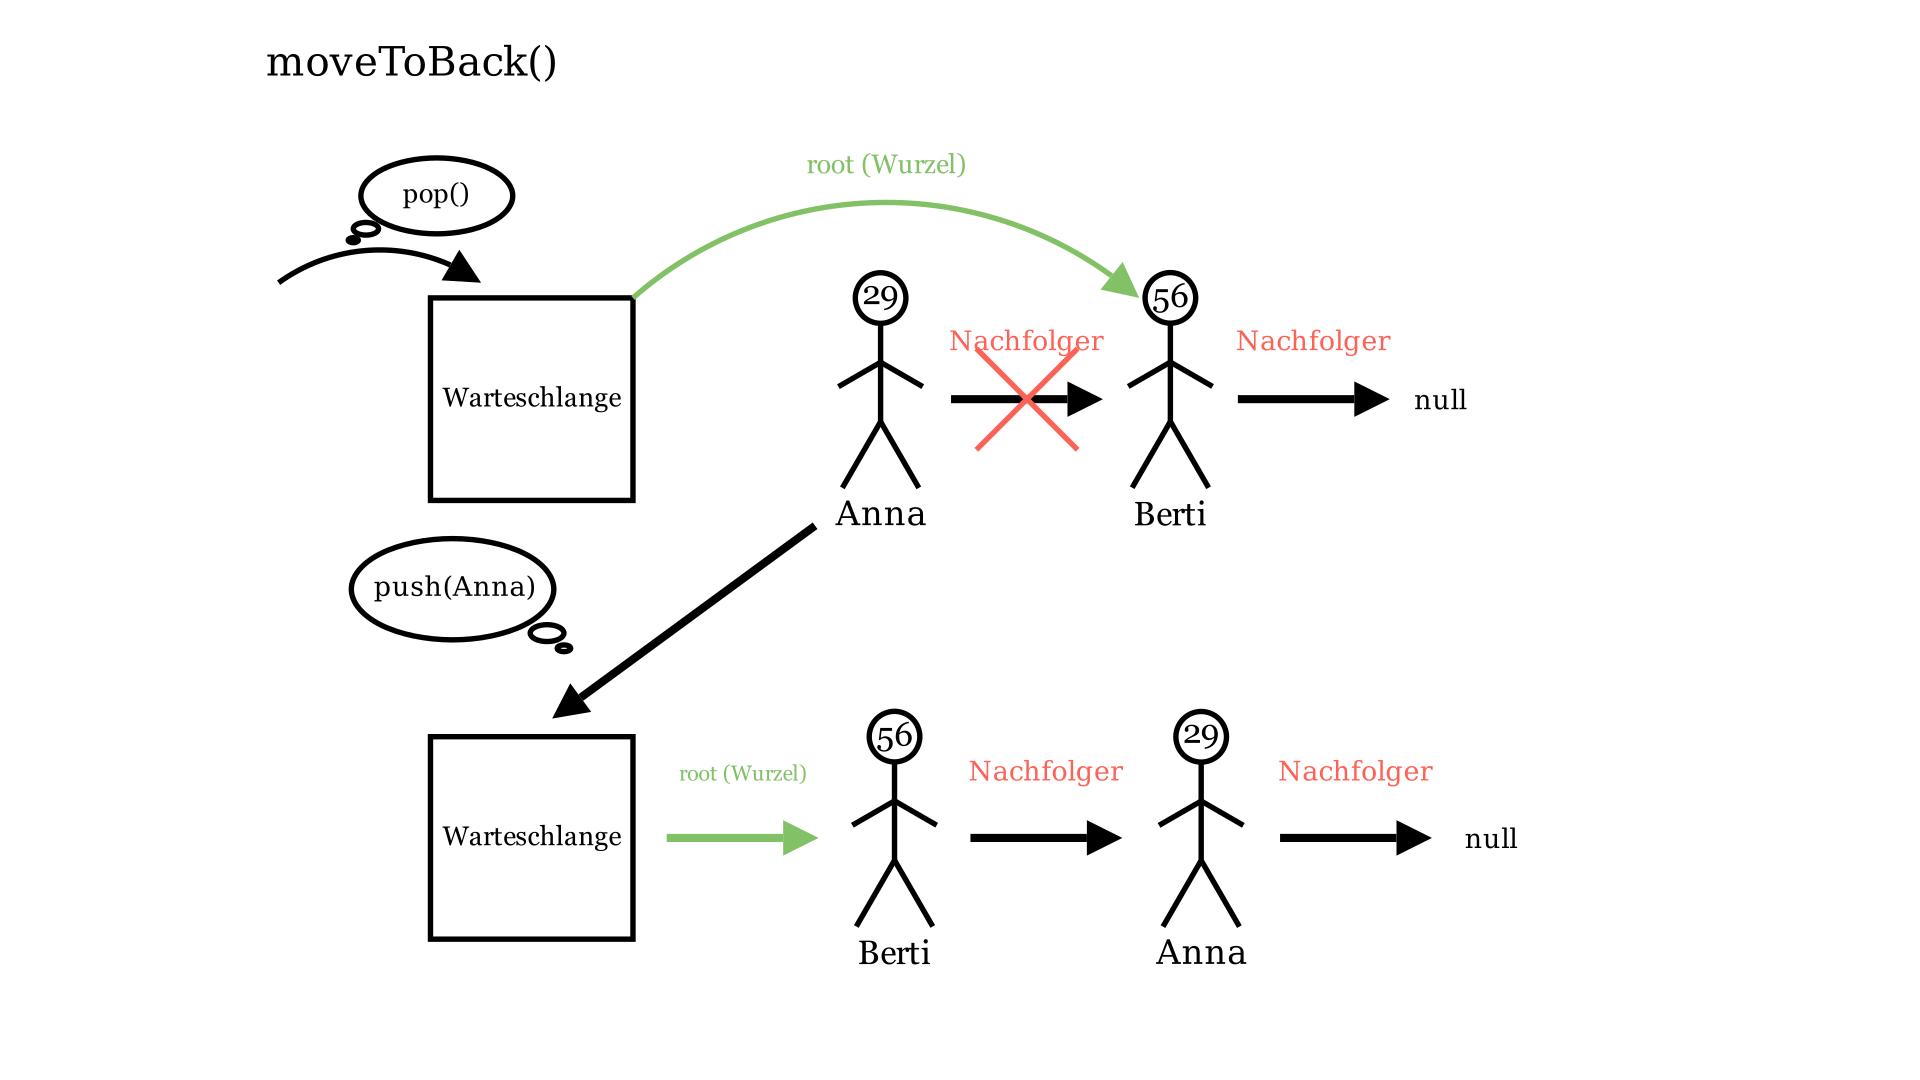
\includegraphics[scale = 0.25]{../../media/linked_moveToBack.png}
\end{center}

\textbf{Aufgabe 3}:
Für diese Aufgabe müssen wir wieder rekursiv denken. Wir können der Warteschlange bzw. der Wurzel nicht direkt sagen, 
zwischen welche beiden Listenelemente die alte Wurzel gesetzt werden muss, da die Wurzel nur die neue Wurzel und 
diese nur ihren Nachfolger kennt. \\
Wir können aber bereits die Länge der Liste bestimmen, d.h. wir können die Methode prüfen lassen, ob das Einfügen 
an dieser Stelle überhaupt möglich ist und andernfalls abbrechen lassen (alternativ könnte dann auch normal 
am Ende eingefügt werden). Außerdem fangen wir ungültige Eingaben ab, die Position 1 wäre die gleiche Stelle wie zuvor,
also wieder die neue Wurzel. Eine negative Eingabe oder 0 macht ebenfalls keinen Sinn. \\
Damit sind die Vorbereitungen abgeschlossen und die alte Wurzel kannt entfernt und in einer lokalen (temporären tmp) 
Variable zwischengespeichert werden. Danach wird die entsprechende Funktion auf der Wurzel aufgerufen und wir wechseln 
in die Mensch-Klasse. \\
Es gibt im Wesentlichen zwei Ideen, wie die entsprechende Position gefunden werden kann:
\begin{enumerate}
    \item Zum Ende laufen und von dort aus in umgekehrter Reihenfolge \q{Durchzählen} ähnlich der Längenbestimmung. (Aufwendig!)
    \item Eine \q{Zählvariable} definieren und mitgeben.
\end{enumerate}
Die zweite Variante ist deutlich einfacher zu implementieren und zu verstehen. In jedem Schritt wird geprüft, ob der 
Zähler eins kleiner als die gewünschte Position ist, damit das ebenfalls mitgegebene Objekt der Klasse Mensch als 
Nachfolger dieses Menschen gesetzt werden kann. Ist diese Position noch nicht erreicht, so wird mit einem um eins erhöhten Zähler
die Methode auf dem nächsten in der Schlange aufgerufen. 

\begin{minted}{Java}
    //class MyListLinked
    public void moveBack(int position) {
        if(position > this.length() || position <= 1) {
            return;
        }
        Human tmp = pop();
        root.moveBack(tmp, position, 1);
    }
    //class Human 
    public void moveBack(Human h, int position, int counter) {
        if(counter == position -1) {
            h.setNext(this.getNext());
            next = h;
        } else {
            next.moveBack(h, position, counter++);
        }
    }
\end{minted}
\textbf{Aufgabe 4}:
Diese Methode durchläuft die Schlange so lange, bis die Nachfolger-Referenz null ist und 
lässt die entsprechenden Informationen mit einem print auf die Konsole schreiben. \\
Die presentation()-Methode ist dabei nicht zwingend nötig und wird nur verwendet, um Ausgabe 
und Logik des Durchlaufs zu trennen. So kann sie leicht verändert werden, ohne dass über den restlichen Code 
nachgedacht werden muss. 
\begin{minted}{Java}
   //class MyListLinked
   public void printList() {
       if(root == null){
           System.out.println("No list here to print!");
       } else {
           root.printList();
       }
   }
   // class Human 
   public void printList(){
      presentation();
      if (next != null) next.printList();
   }
   public void presentation(){
        System.out.println("I am " + name + " and I am " + age + " years old");
   }
\end{minted}
\textbf{Aufgabe 5}:
Die grundlegende Idee der Methode verändert sich durch diese Änderung nicht, allerdings 
muss jeder Mensch seine Informationen an den String anhängen, d.h. an jedem Menschen 
in der Warteschlange wird ein String erzeugt und anschließend der nächste Mensch 
nach seinen Informationen \q{gefragt}, indem auf dem Nachfolger wiederum die printList()-
Methode aufgerufen wird. \\
Der Befehl \textbackslash n erzeugt eine neue Zeile, andernfalls würde der String nur eine lange
Zeile ergeben, wenn man ihn weiterverwendet und ausgibt. 
\begin{minted}{Java}
   //class MyListLinked
   public String printList() {
       if(root == null){
           System.out.println("No list here to print!");
           return "";
       } else {
           return root.printList();
       }
   }
   // class Human 
   public String printList(){
    String toReturn = "I am " + name + " and I am " + age + " years old";
      if (next != null){
        return toReturn + "\n" + next.printList()
      } 
      return toReturn;
   }

\end{minted}
\textbf{Aufgabe 6}:
Für diese Methode wird wieder der rekursive Aufbau der Liste genutzt, im Wesentlichen entspricht die 
Logik der moveBack() - Methode. Wir benötigen wieder einen Zähler für die Such-Methode in der 
Klasse Mensch, da die einzelnen Menschen ihre Position nicht kennen und wir mitzählen müssen. \\
Die Festlegung, dass $-1$ zurückgegeben wird, wenn das Element nicht in der Liste ist, ist 
wieder willkürlich festgelegt, andere Lösungen sind denkbar. 
\begin{minted}{Java}
    //class MyListLinked   
    public int searchHumanInQueue(Human human) {
        int counter = 0;
        int searched = root.searchHumanInQueue(human,counter);
        return searched;
    }
    //class Human 
    public int searchHumanInQueue(Human human, int counter){
        if(human.equals(this)){
            return counter;
        } 
        if(next != null) {
            return next.searchHumanInQueue(human, counter+1);
        } else {
            return -1;
        }
    }
\end{minted}
\textbf{Aufgabe 7}:
Die Struktur der Funktion ist wieder dieselbe, diesmal sogar ohne eine Zählvariable. Soll die rekurisve 
Methode nicht implementiert werden, kann auch wieder auf die Methode aus Aufgabe 6 zurückgegriffen 
werden. 
\begin{minted}{Java}
    //class MyListLinked 
    public boolean contains(Human human) {
        if(root != null) {
            return root.contains(human);
        } else {
            return false;
        }

    }
    //class Human
    public boolean contains(Human human) {
        if(human.equals(this)) {
            return true;
        } else {
            if(next != null){
                return next.contains(human);
            } else {
                return false;
            }
            
        }
    }
    //Alternatively use searchHumanInQueue()!
\end{minted}
\textbf{Aufgabe 8}: 
Für diese Methode kann wieder auf die Struktur von Aufgabe 3 zurückgegriffen werden. Auch hier
empfiehlt es sich, die Referenz auf den nächsten Menschen in der Liste vor der Rückgabe wieder zu entfernen, 
da sonst \q{von außerhalb} die Liste modifiziert werden könnte. Wird die erste Position gewählt, so kann einfach die vorneEntfernen-Methode verwendet werden. 
\begin{minted}{Java}
    //class MyListLinked
    public Human removeAt(int position) {
        if(position == 1) {
            return pop();
        }
        if(root != null) {
            int counter = 1;
            return root.removeAt(position, counter);
        } else {
            return null;
        }
    }
    //class Human 
    public Human removeAt(int position, int counter){
        if(next == null) {
            return null;
        }
        if(counter == position - 1) {
            Human tmp = next;
            next = next.getNext();
            return tmp;
        } else {
            return next.removeAt(position, counter + 1);
        }
    }

\end{minted}
\textbf{Aufgabe 9}:
Im Gegensatz zur Feld-Implementierung ist das Zusammenfügen zweier Listen mit der 
verketteten Struktur denkbar einfach. Es muss lediglich das letzte Element der ersten 
Liste gefunden werden (hier über eine Helfer-Methode, die die Liste durchläuft und 
immer prüft, ob das nächste Element gleich null ist) und das erste Element der zweiten Liste
als dessen Nachfolger gesetzt werden. Alternativ kann auch das erste Element der zweiten Liste mit 
Hilfe der push-Methode angefügt werden. 
\begin{minted}{Java}
    //class MyListLinked
    public Object concatenate(MyListLinked toConcat) {
        if(root == null) {
            return toConcat;
        }
        Human end = this.findEnd();
        end.setNext(toConcat.getRoot());
        return this;
    }
    //class Human
    public Human findEnd(){
        if(next == null) {
            return this;
        } else {
            return next.findEnd();
        }
    }
\end{minted}
\end{document}